\documentclass{sprawozdanie-agh}
\title{IO - dolina narciarska}
\usepackage{lscape}
\usepackage[final]{pdfpages}
\usepackage[utf8]{inputenc}
\usepackage{listings}
\usepackage{geometry}
\usepackage{lscape}
\geometry{
 a4paper,
 total={170mm,257mm},
 left=20mm,
 right=20mm,
 top=20mm,
}

\makeatletter

\begin{document}

\przedmiot{Inżynieria Oprogramowania}
\tytul{Projekt systemu \\ doliny narciarskiej \textit{Łojezusicku}}
\podtytul{...}
\kierunek{Informatyka}
\autor{Patryk Gałczyński, Szymon Duda}
\data{Kraków, 4 grudnia 2016}

\stronatytulowa{}

\section{Krótki opis systemu}
    \large
    Nasz projekt zakłada zamodelowanie działania kompleksu narciarskiego. Nasza stacja narciarska będzie oferować możliwość zakupu karnetów w kasie badź online. Klient będzie miał możliwość dokonania płatności gotówką, kartą lub przelewem. Do wyboru będzie miał różne metody potwierdzenia płatności, faktura, paragon. W naszej ofercie znajdą się karnety czasowe oraz "na punkty". Dla młodych narciarzy oraz grup zorganizowanych przygotowaliśmy specjalną ofertę zniżkową. Karnet czasowy umożliwia korzystanie ze wszystkich wyciągów w obrębie naszego kompleku w danym okresie, karnet punktowy pozwala na korzystanie z wyciągów do wyczerpania posiadanej ilości punktów na karnecie, przy czym, skorzystanie z określonego wyciągu redukuje ilość punktów na karcie o daną ilość, dla każdego wyciągu zdefiniowaną indywidualnie. Klient będzie musiał wypożyczyć kaucjonowaną kartę magnetyczną lub przypisać karnet do legitymacji z chipem. W ramach funkcjonowania całego kompleksu narciarskiego, klient będzie miał możliwość wynajęcia instruktora, oraz całego potrzebnego sprzętu w lokalnej wypożyczalni. W obrębie wypożyczalni będzie działać rówież serwis, gdzie klient będzie mógł zlecić renowację własnego sprzętu.

\section{Lista bodźców zewnętrznych}
    \begin{enumerate}
	\item żądanie kupna karnetu
        \item żądanie zwrotu nie używanego karnetu
        \item żądanie sprawdzenia stanu punktowego karnetu
        \item żądanie realizacji płatnośći
	\item żądanie wyboru metody potwierdzenia zakupu
	\item żądanie przypisania karnetu do karty (kaucjonowana lub legitymacja)
	\item żądanie zwrotu karty kaucjonowanej
	\item żądanie przeniesienia nieużytego karnetu na inny dzień
	\item żądanie rezerwacji instruktora
        \item żądanie wypożyczenia sprzetu
	\item żądanie oddania wypożyczonego sprzętu
	\item żądanie zlecenia serwis sprzętu
	\item żądanie zwrotu serwisowanego sprzętu
    \end{enumerate}

\newpage
\section{Diagram przepływu danych}
\begin{center}
    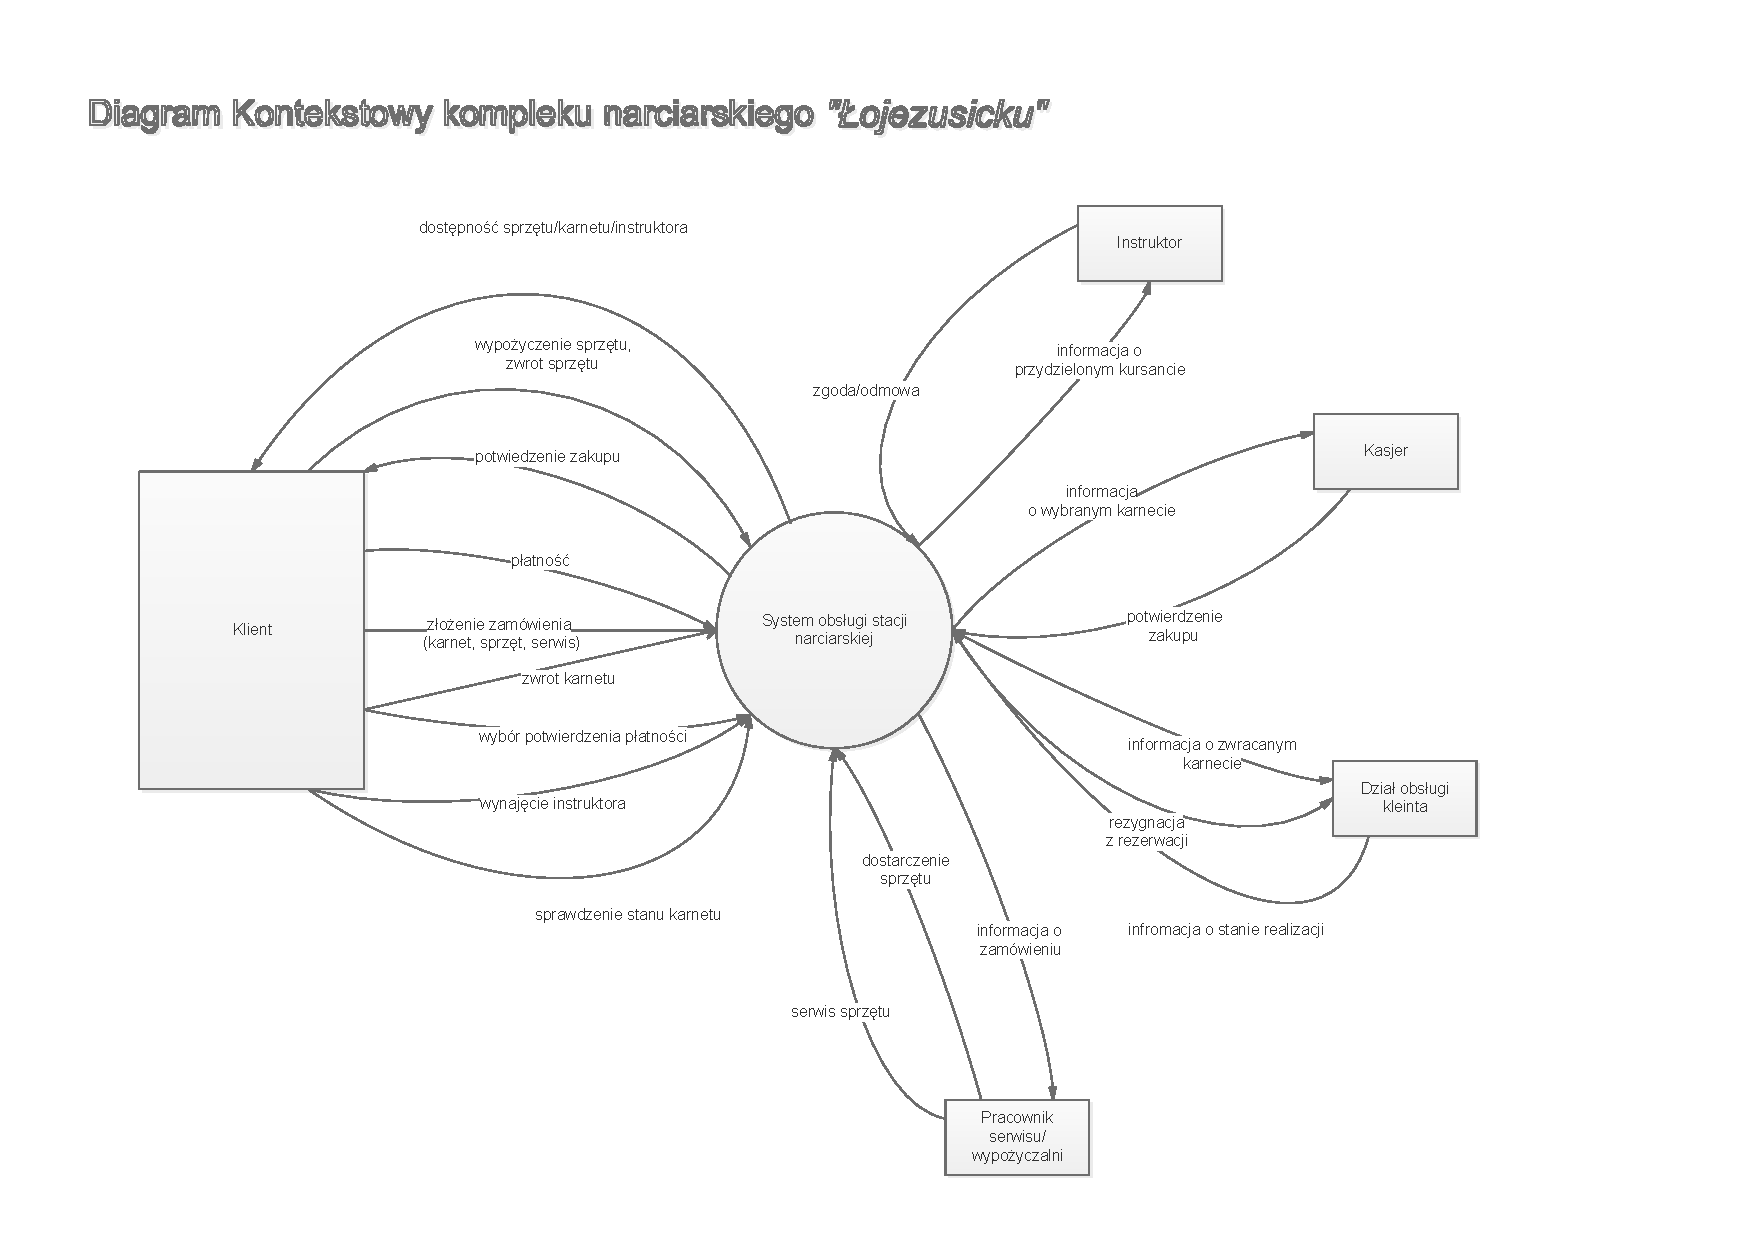
\includegraphics[scale=0.25]{diagram_kontekstowy}
\end{center}

\begin{landscape}
    \newpage
    \section{Diagram przepływu danych - poziom 0}
    \begin{figure}
        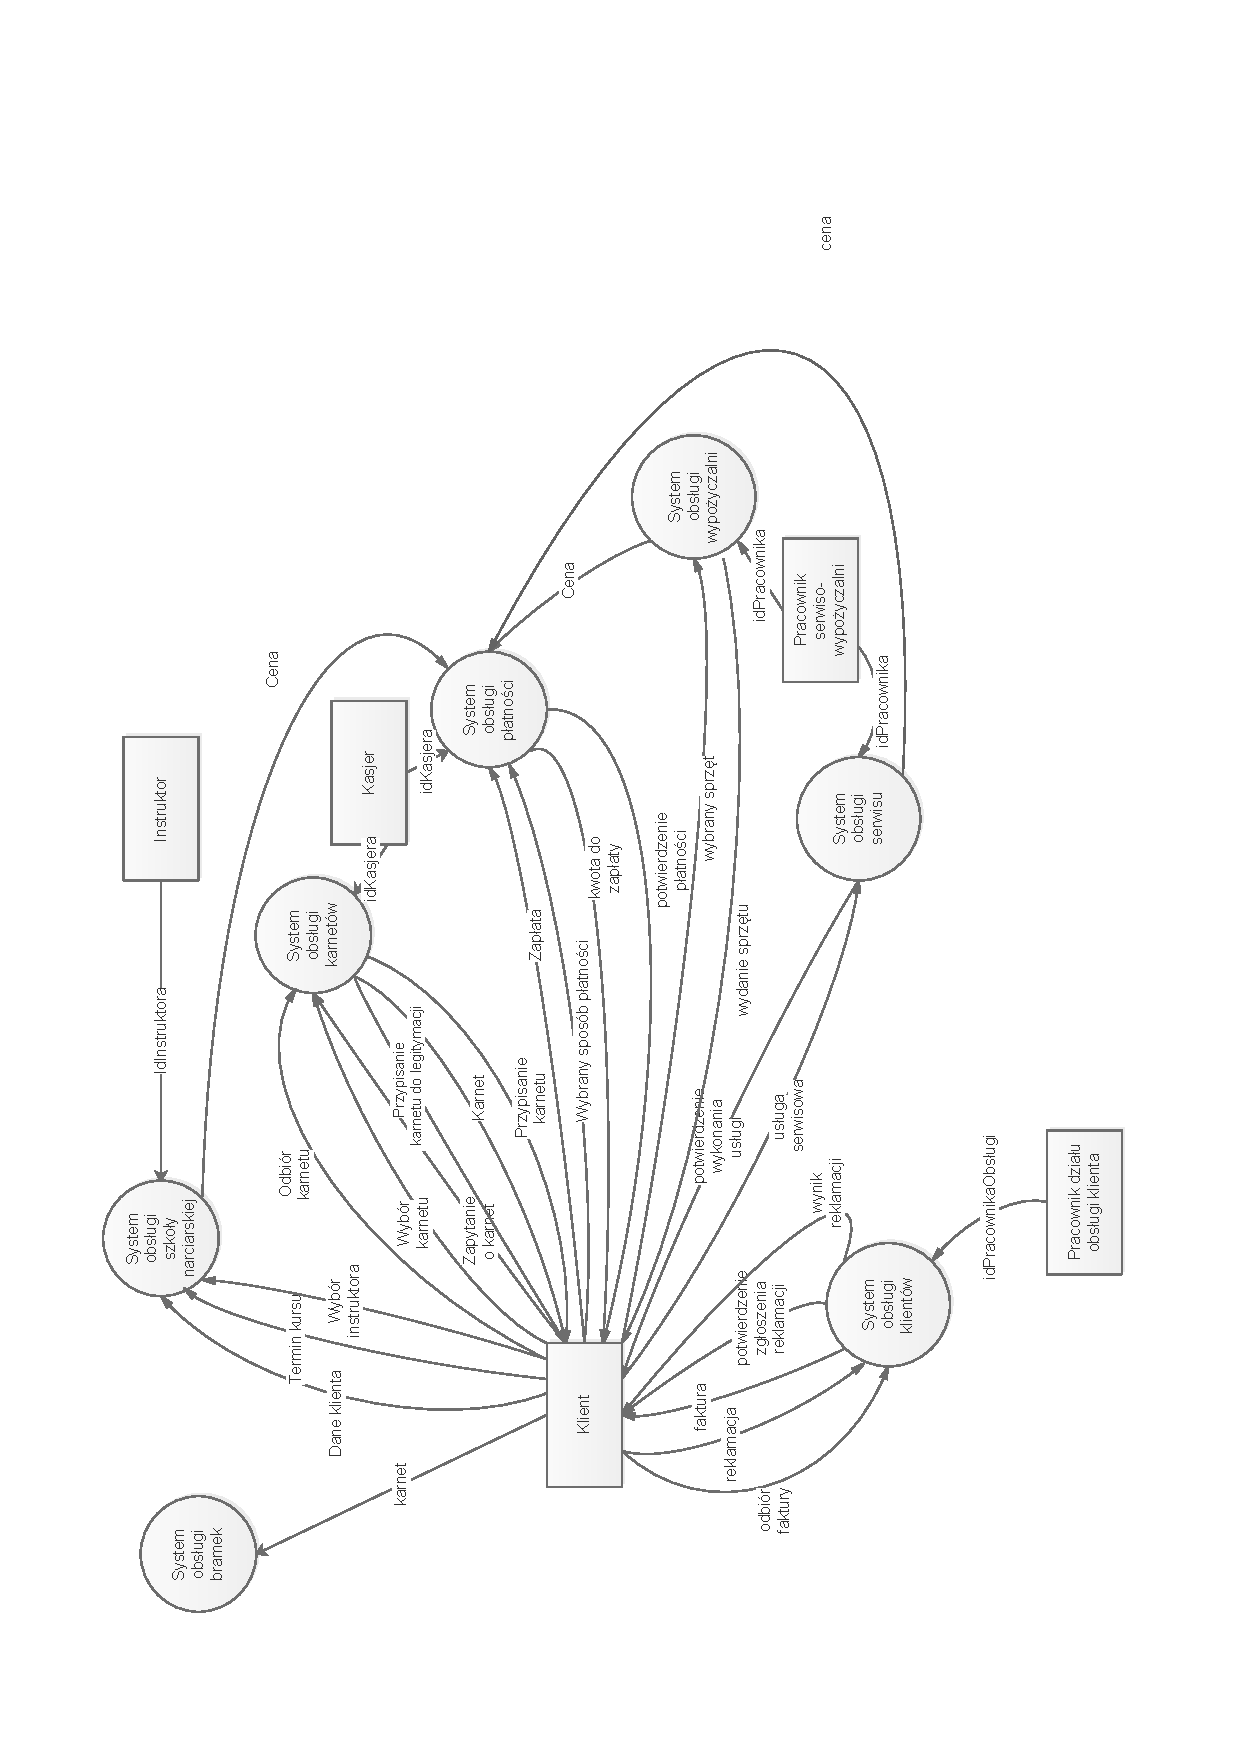
\includepdf[trim=-3cm 0 0 0]{dfd/p0/p0-all-rotated-2}
    \end{figure}

\newpage
\section{Diagram przepływu danych - poziom 1}
\subsection{Kasa biletowa}
\begin{figure}
    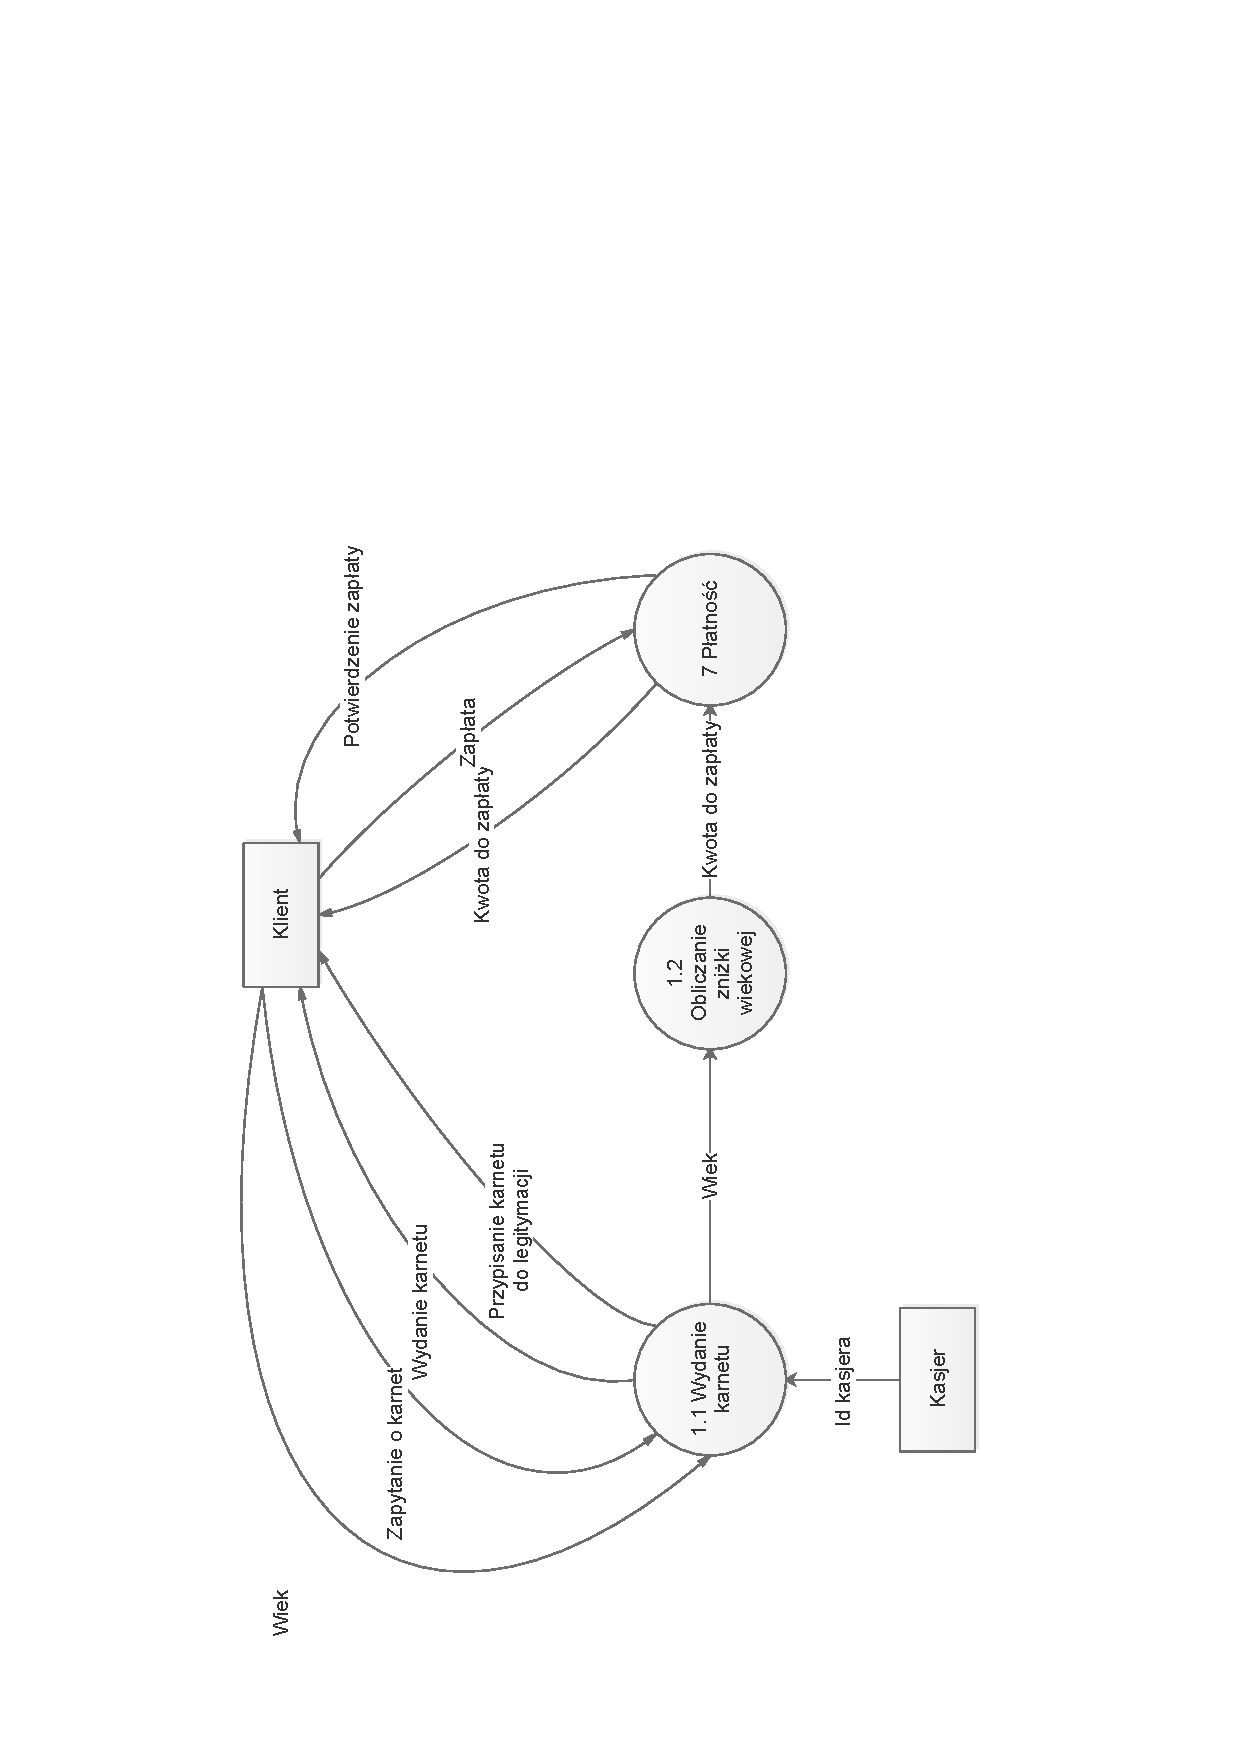
\includepdf[trim=-3cm 0 0 0]{dfd/p1/p1-kasabiletowa-rotated}
\end{figure}

\newpage
\subsection{Obsługa klienta}
\begin{figure}
    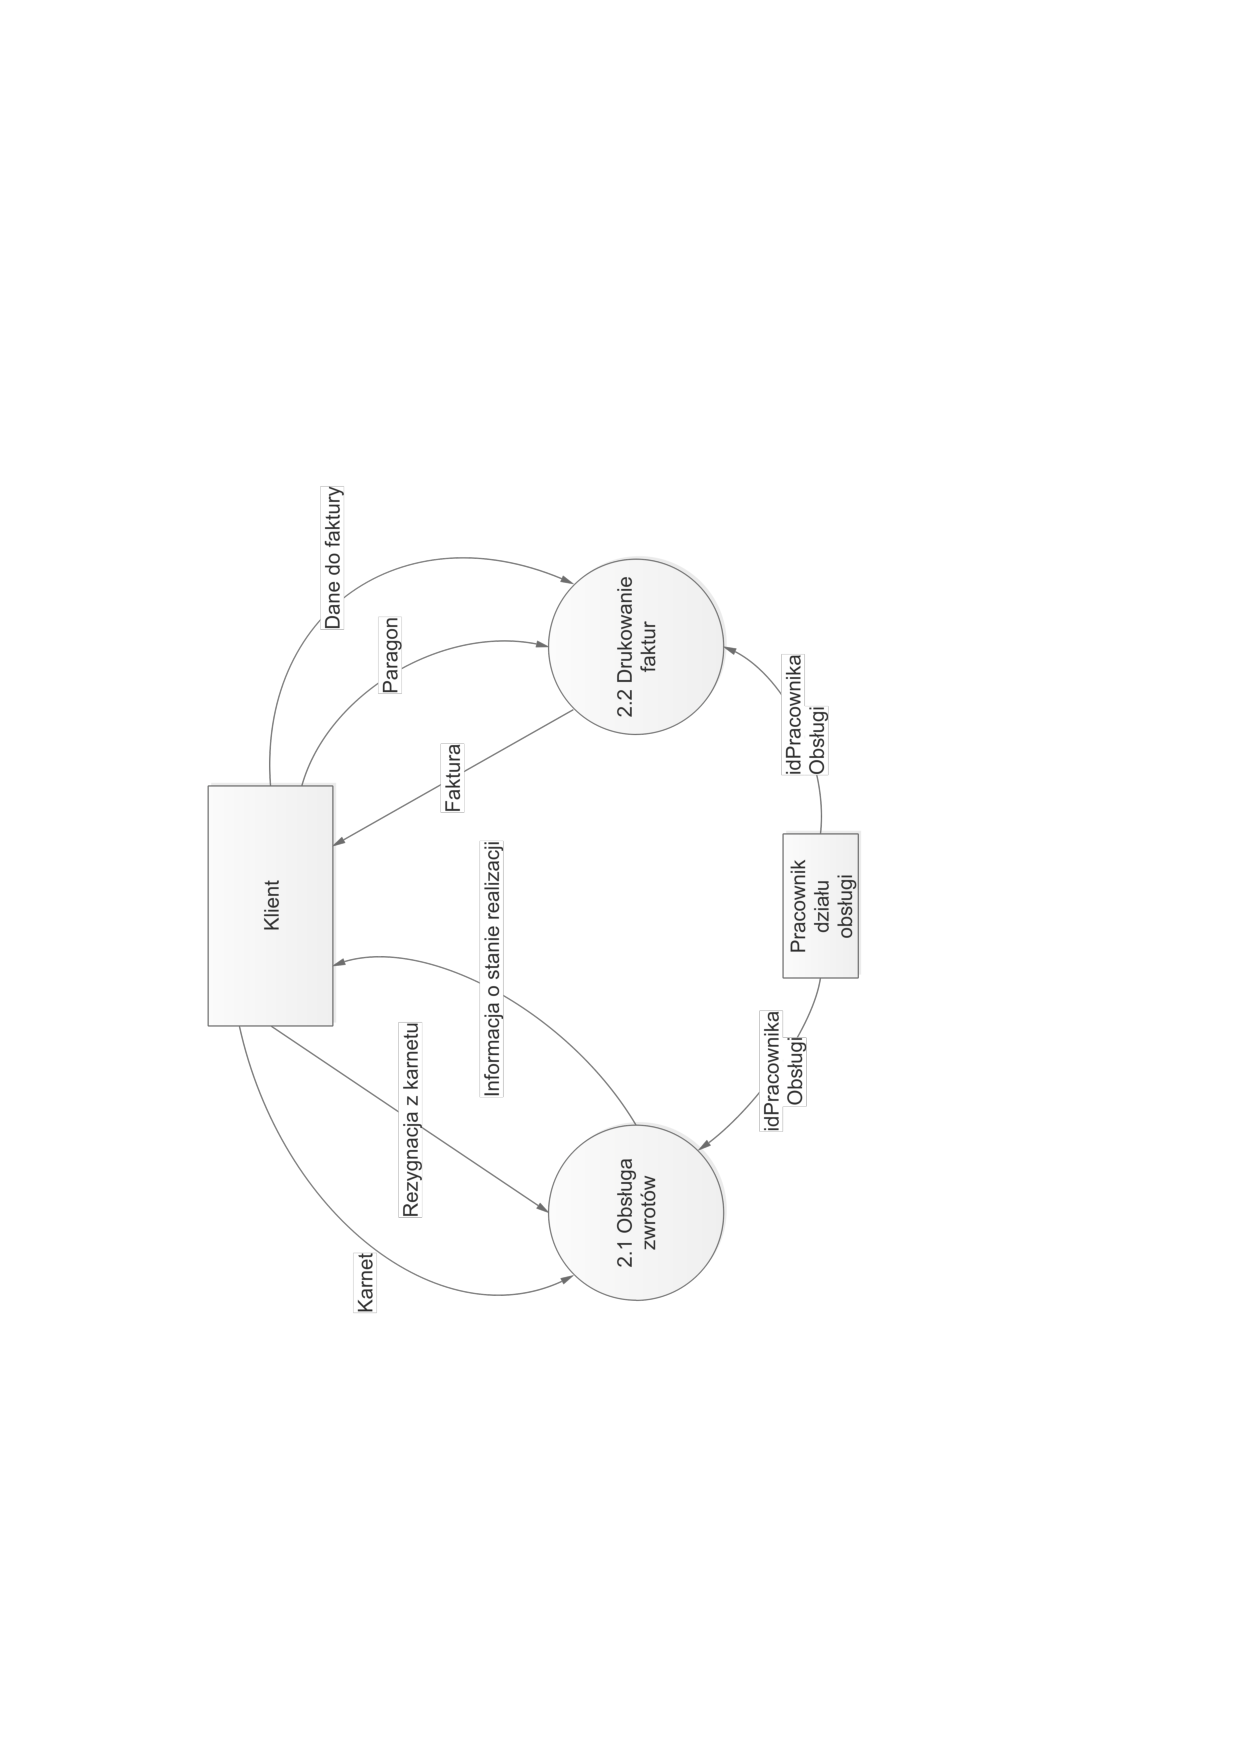
\includepdf[trim=-3cm 0 0 0]{dfd/p1/p1-dzialobslugi-rotated}
\end{figure}

\newpage
\subsection{Szkółka narciarska}
\begin{figure}
    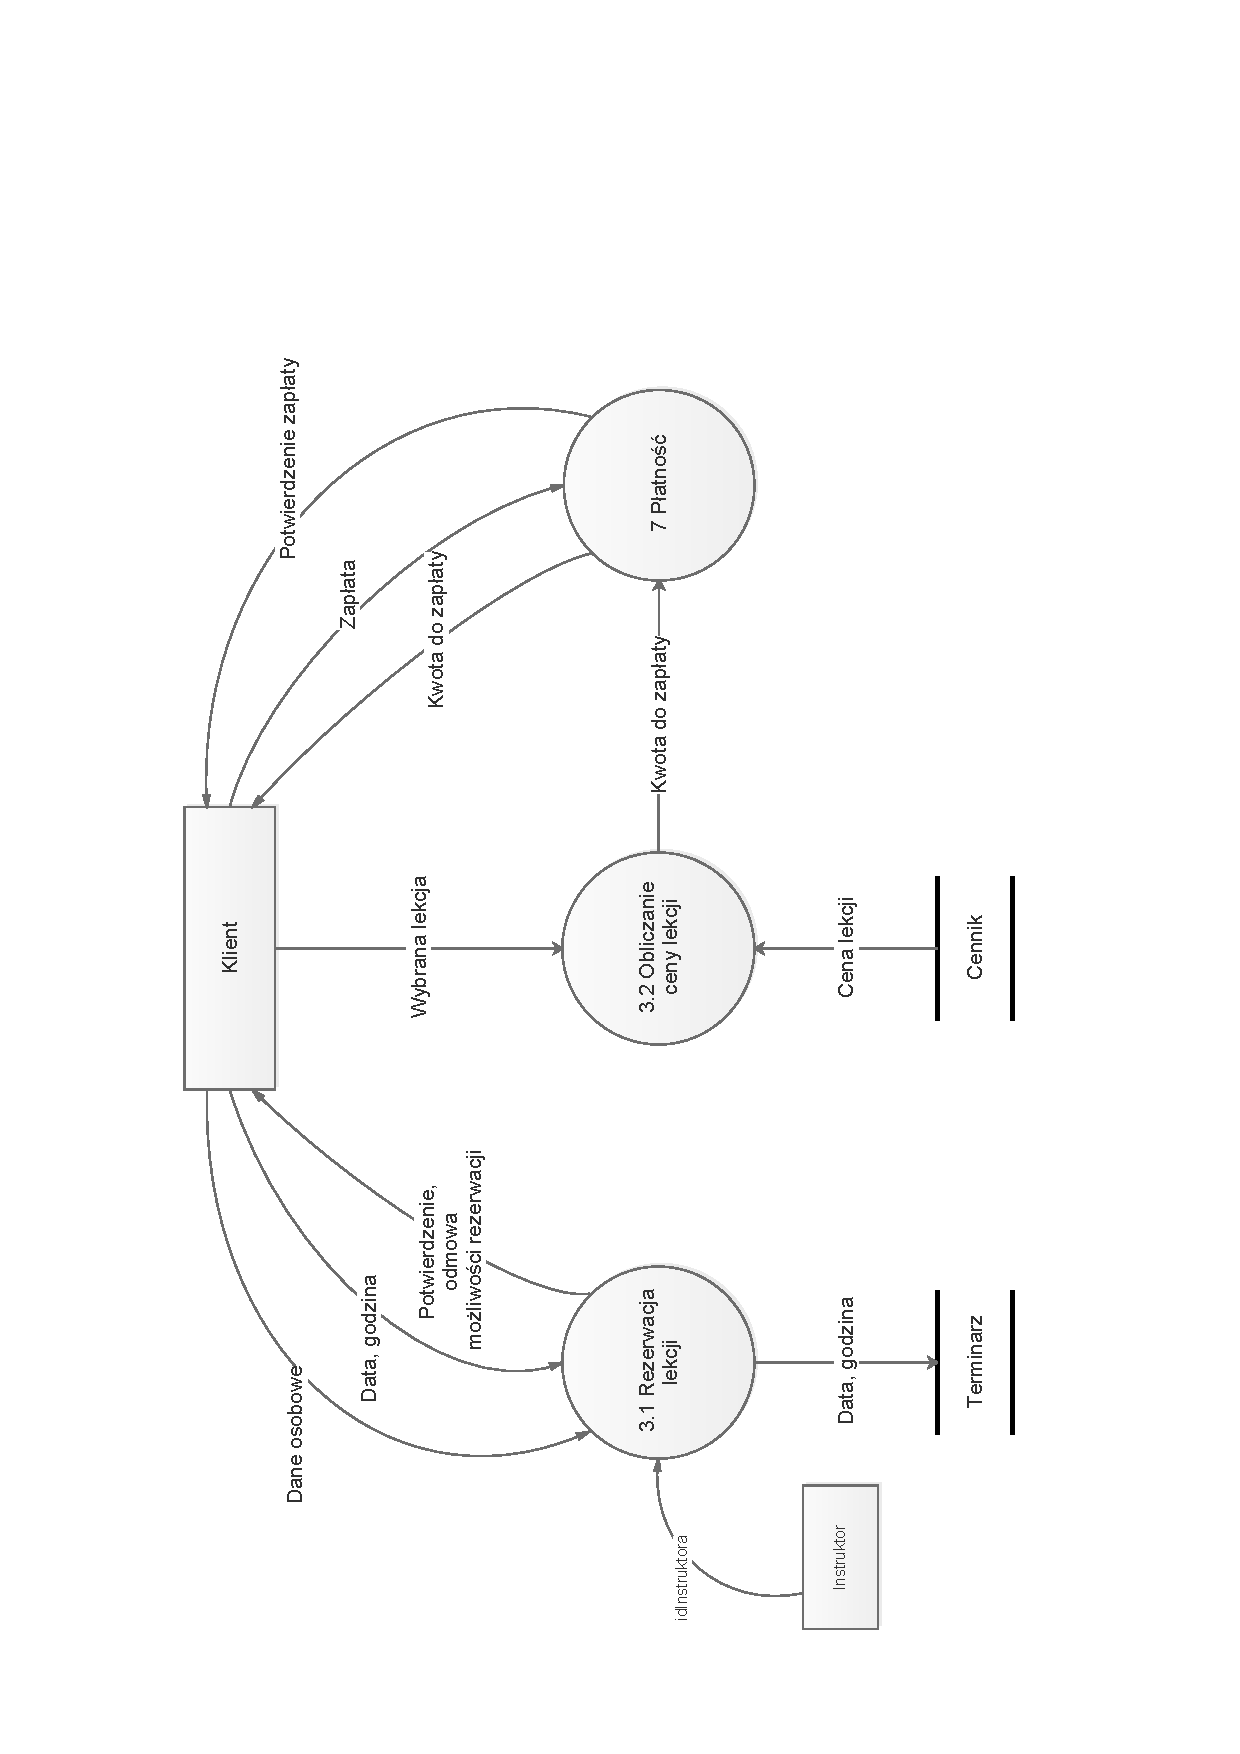
\includepdf[trim=-3cm 0 0 0]{dfd/p1/p1-szkola-rotated}
\end{figure}

\newpage
\subsection{Wypożyczalnia sprzętu}
\begin{figure}
    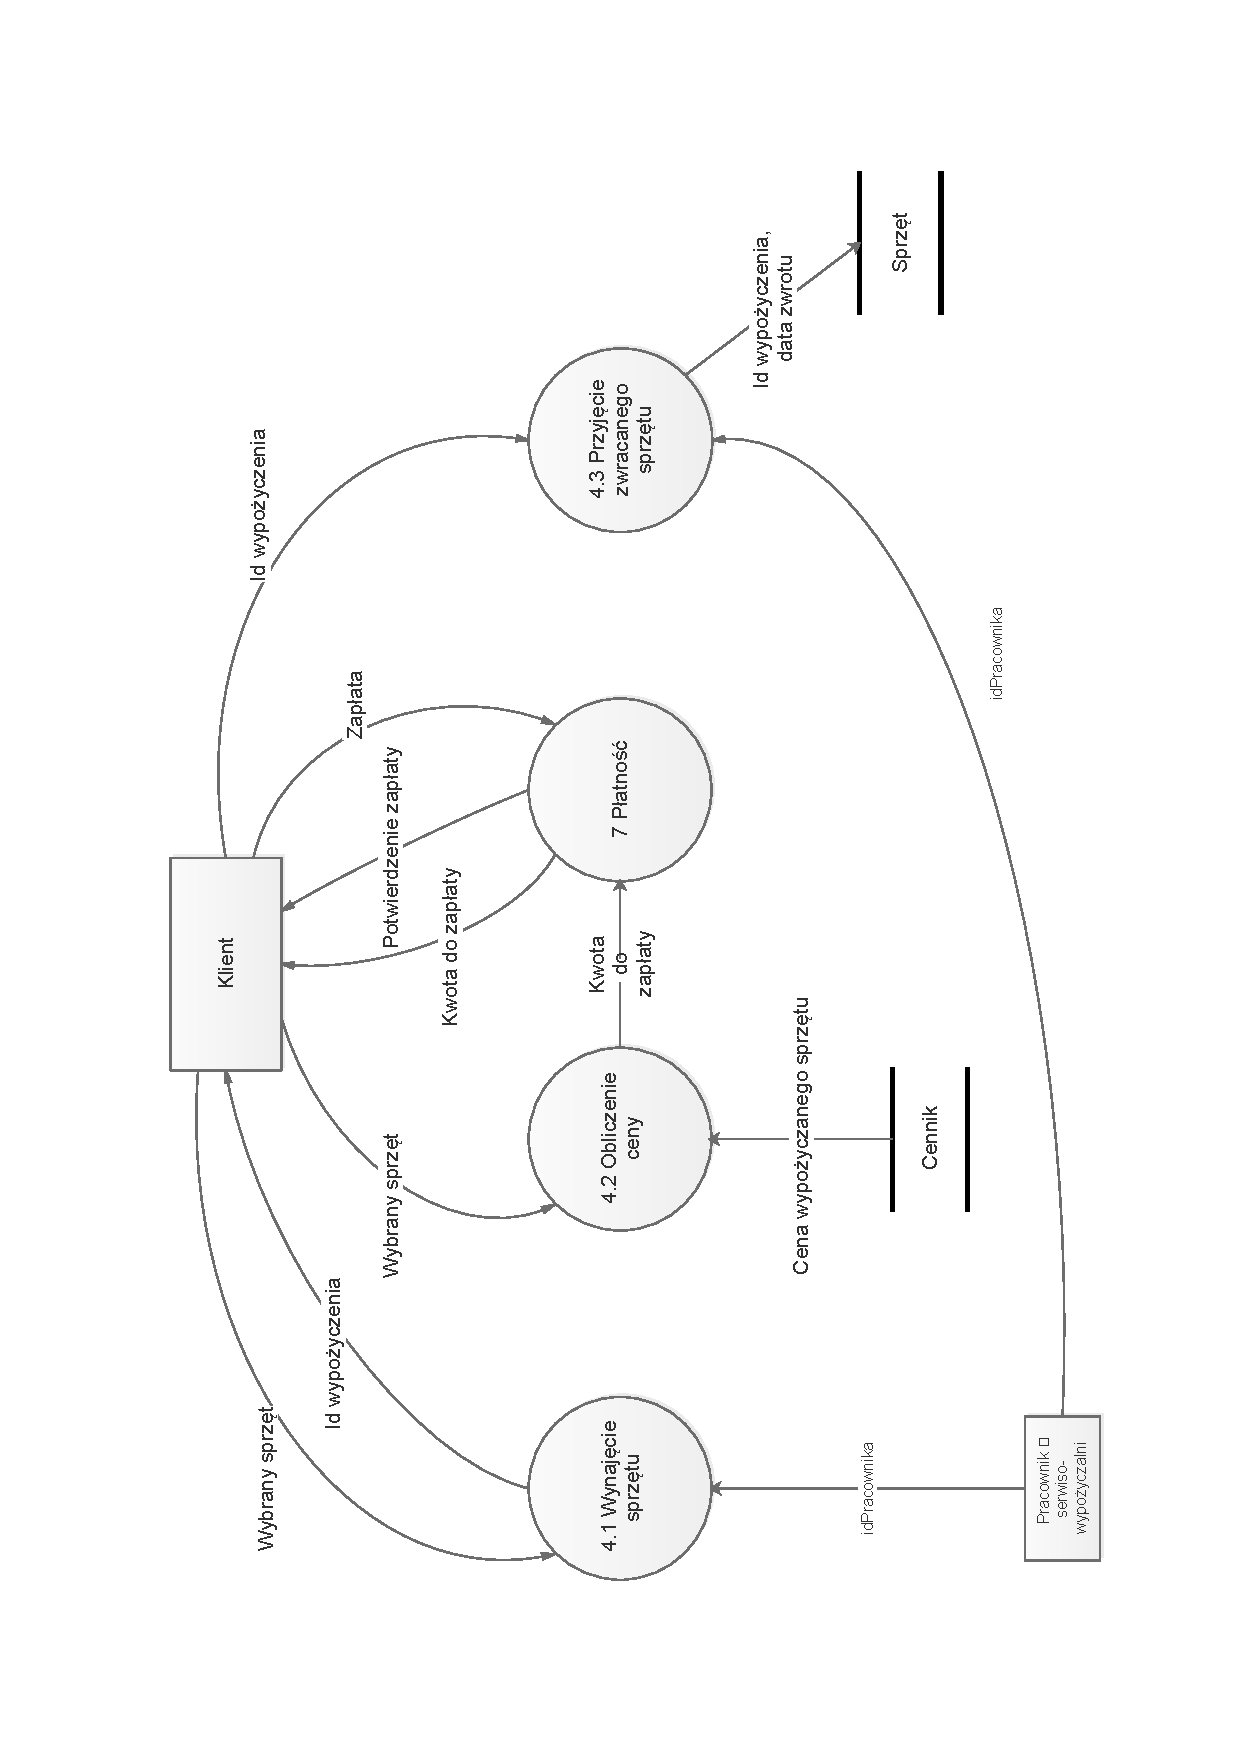
\includepdf[trim=-3cm 0 0 0]{dfd/p1/p1-wypozyczalnia-rotated}
\end{figure}

\newpage
\subsection{Serwis sprzętu}
\begin{figure}
    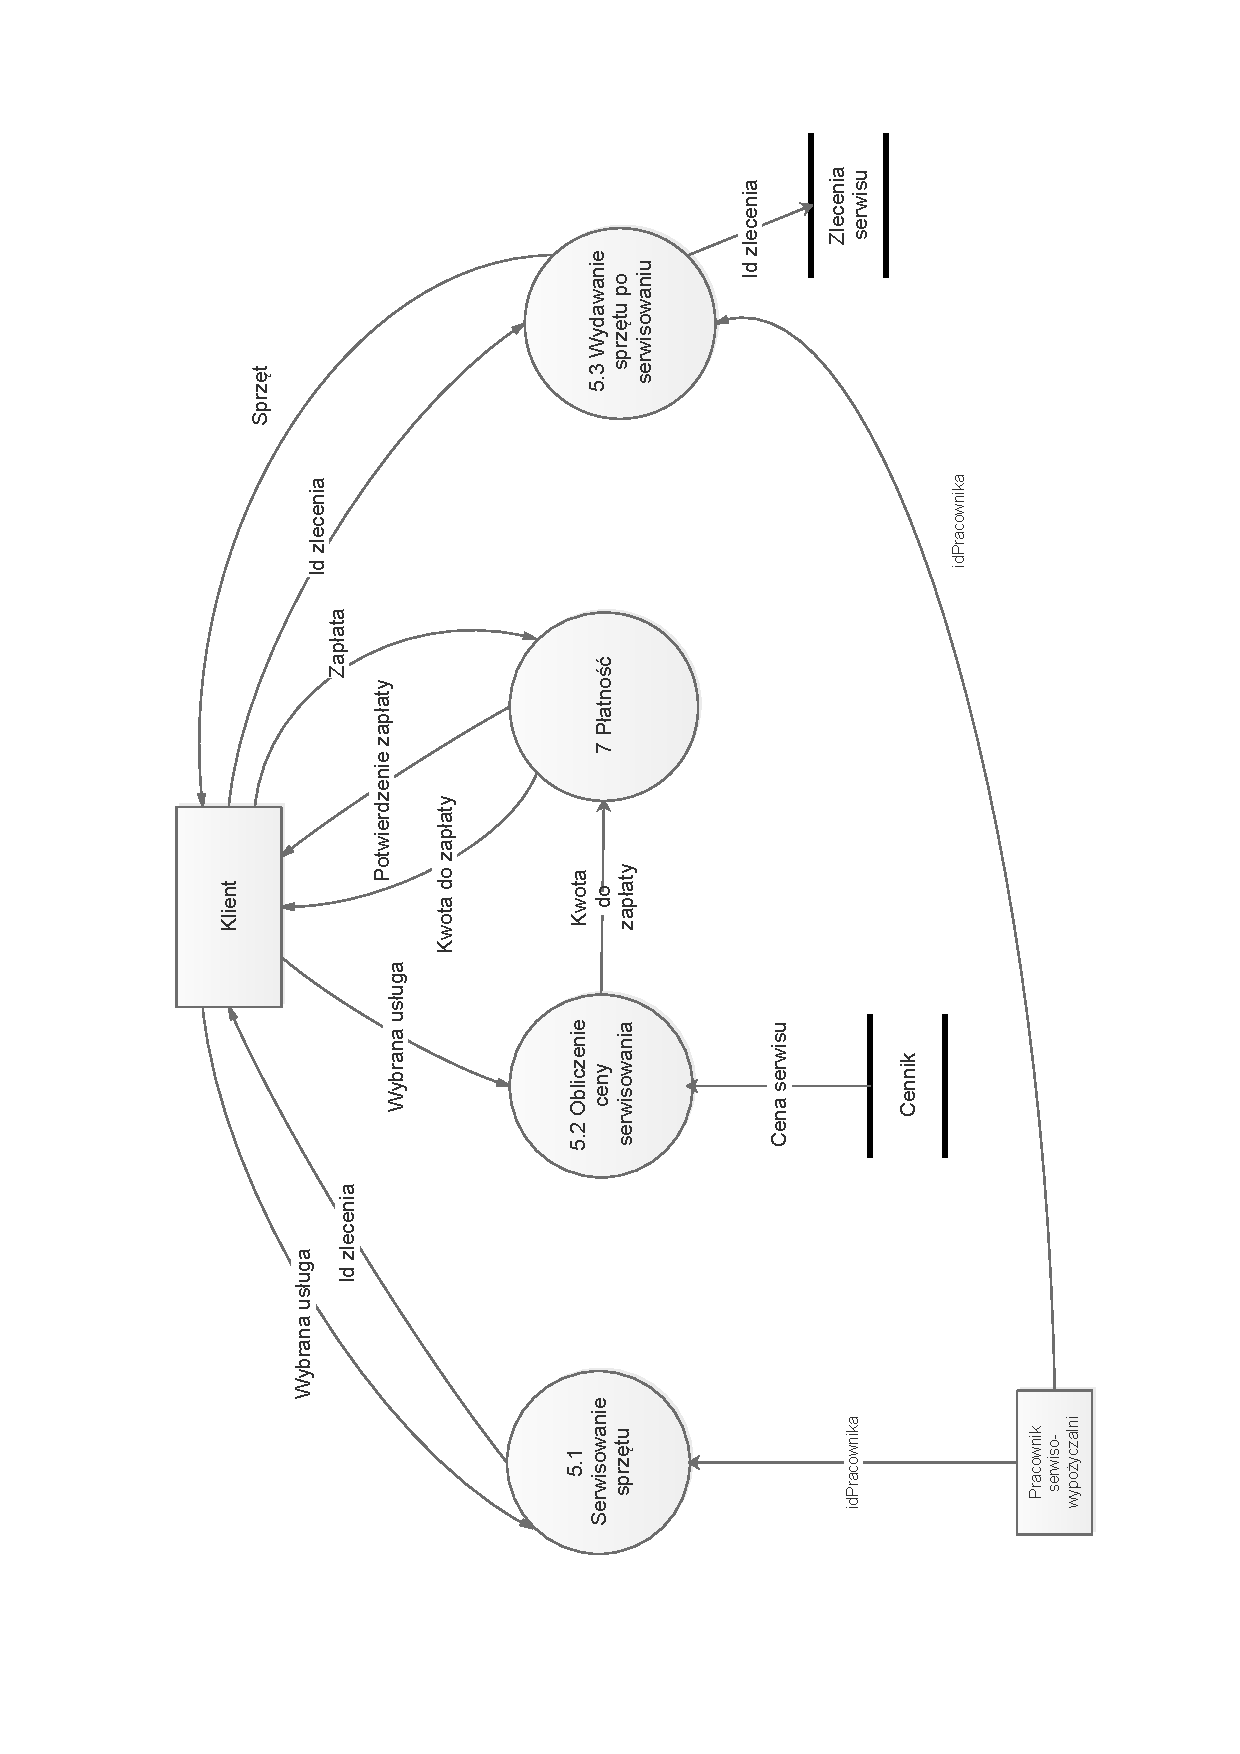
\includepdf[trim=-3cm 0 0 0]{dfd/p1/p1-serwis-rotated}
\end{figure}

\newpage
\subsection{Bramki}
\begin{figure}
    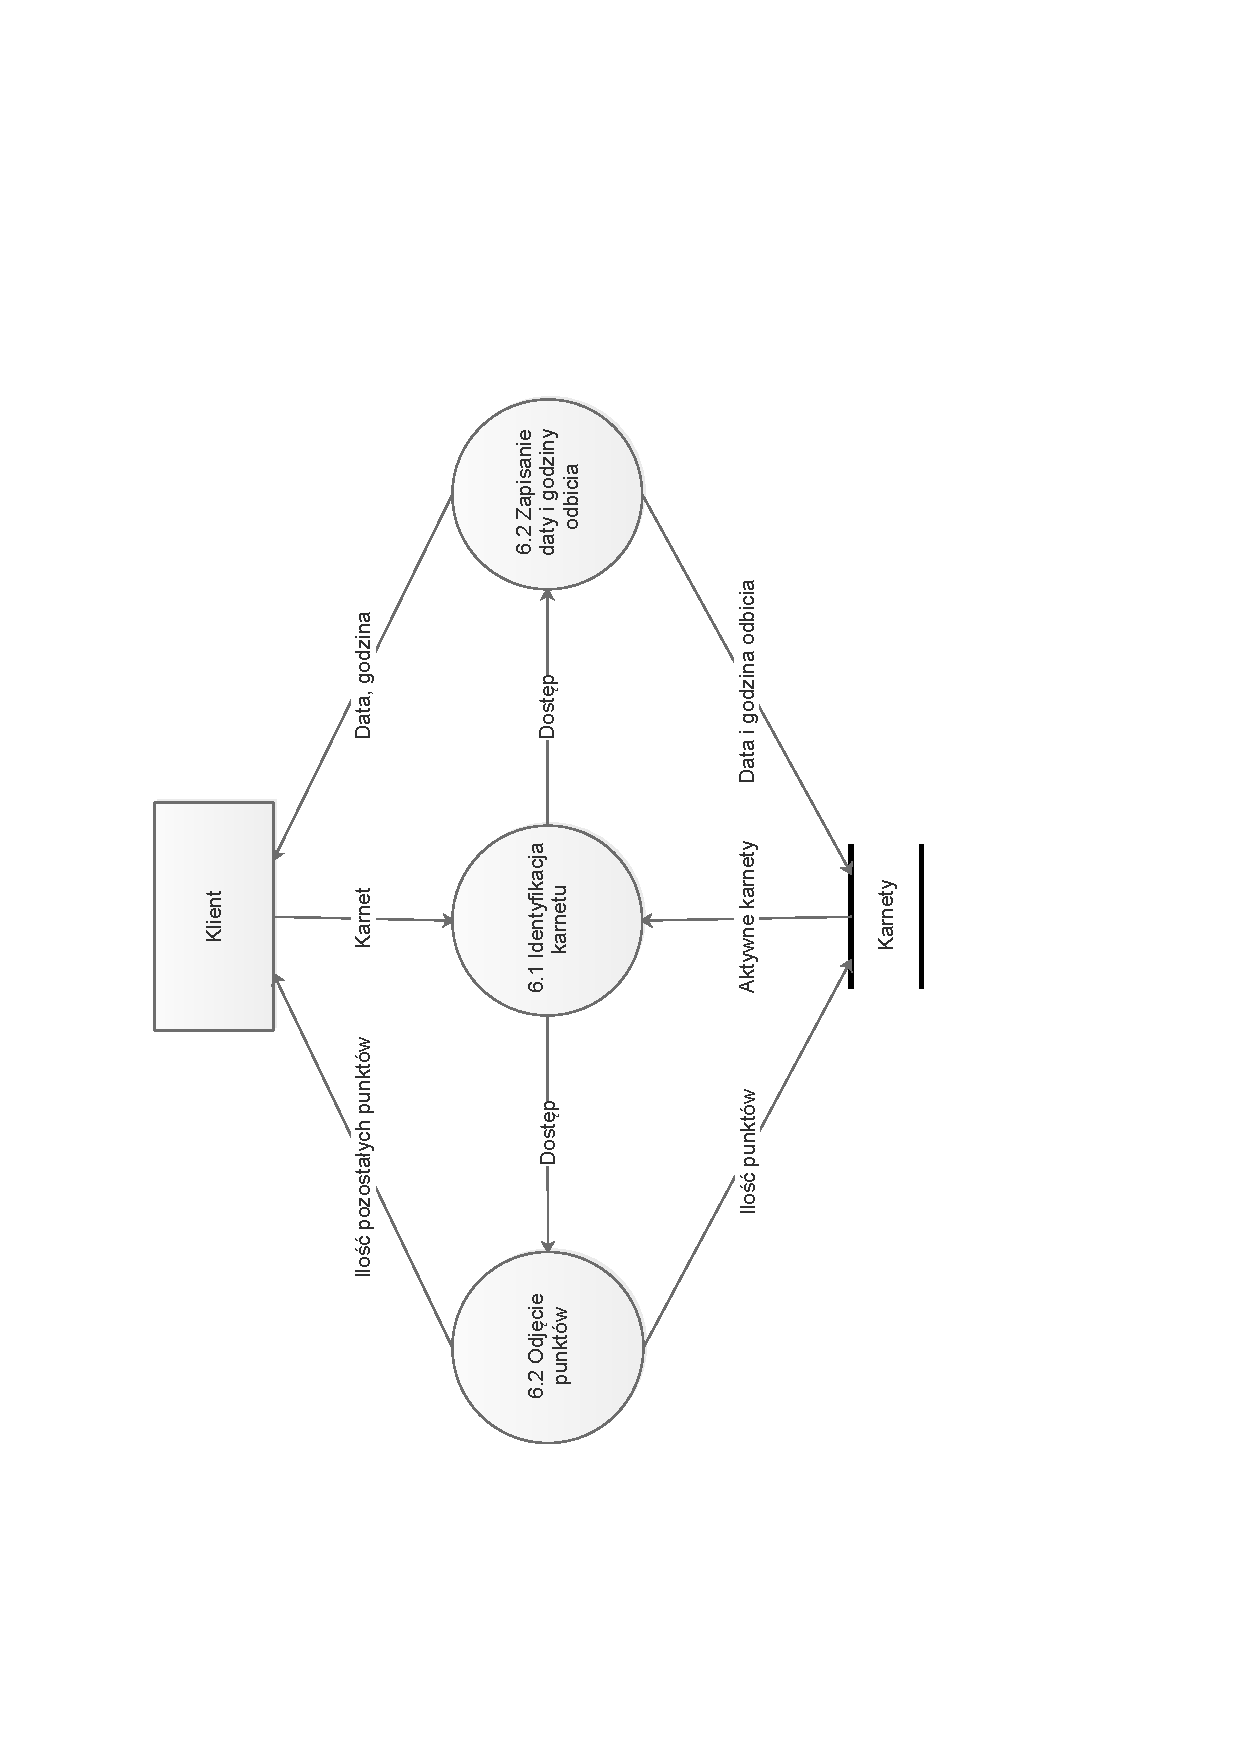
\includepdf[trim=-3cm 0 0 0]{dfd/p1/p1-bramki-rotated}
\end{figure}

\newpage
\section{Diagram przepływu danych - poziom 2}
\subsection{Kasa biletowa - kupno karnetu}
\begin{figure}
    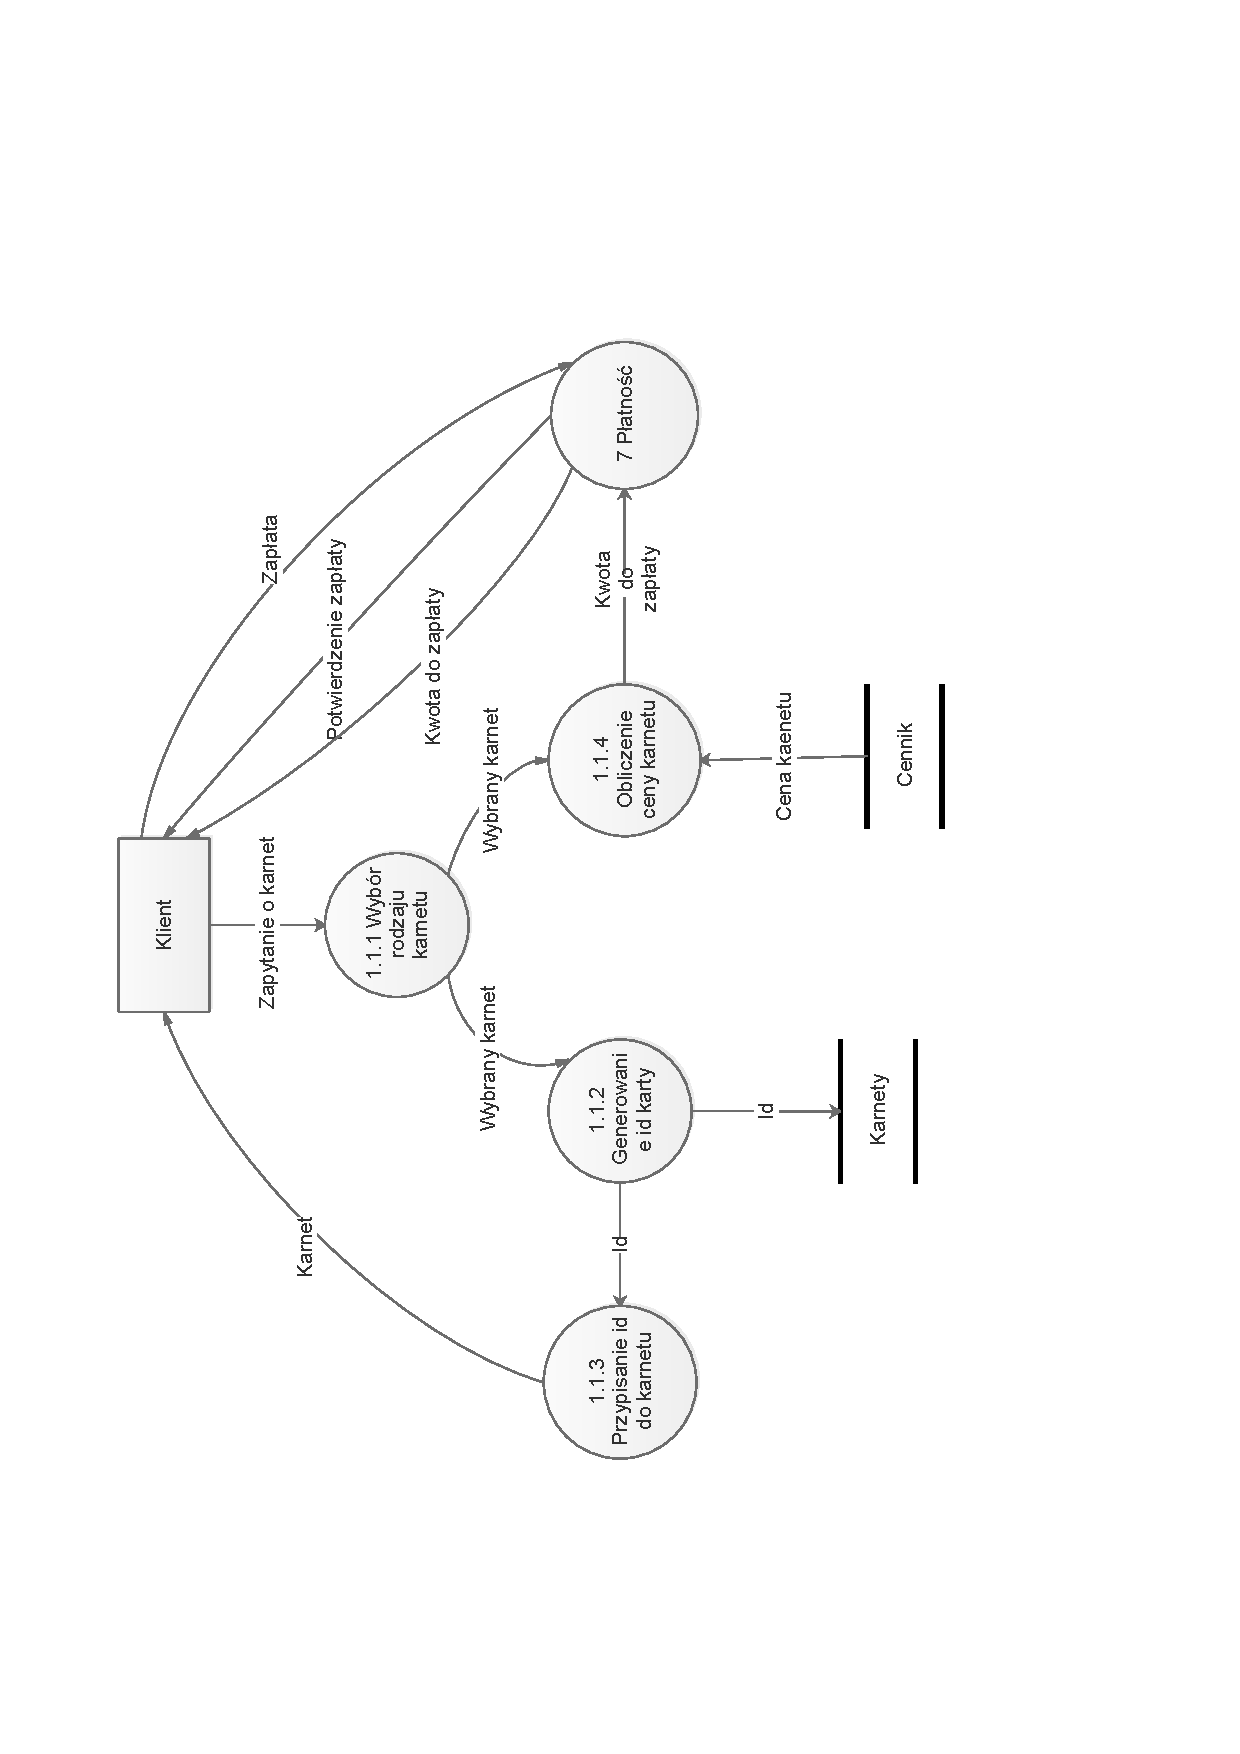
\includepdf[trim=-3cm 0 0 0]{dfd/p2/p2-kupnokarnetu-rotated}
\end{figure}

\newpage
\subsection{Obsługa klienta - zwroty}
\begin{figure}
    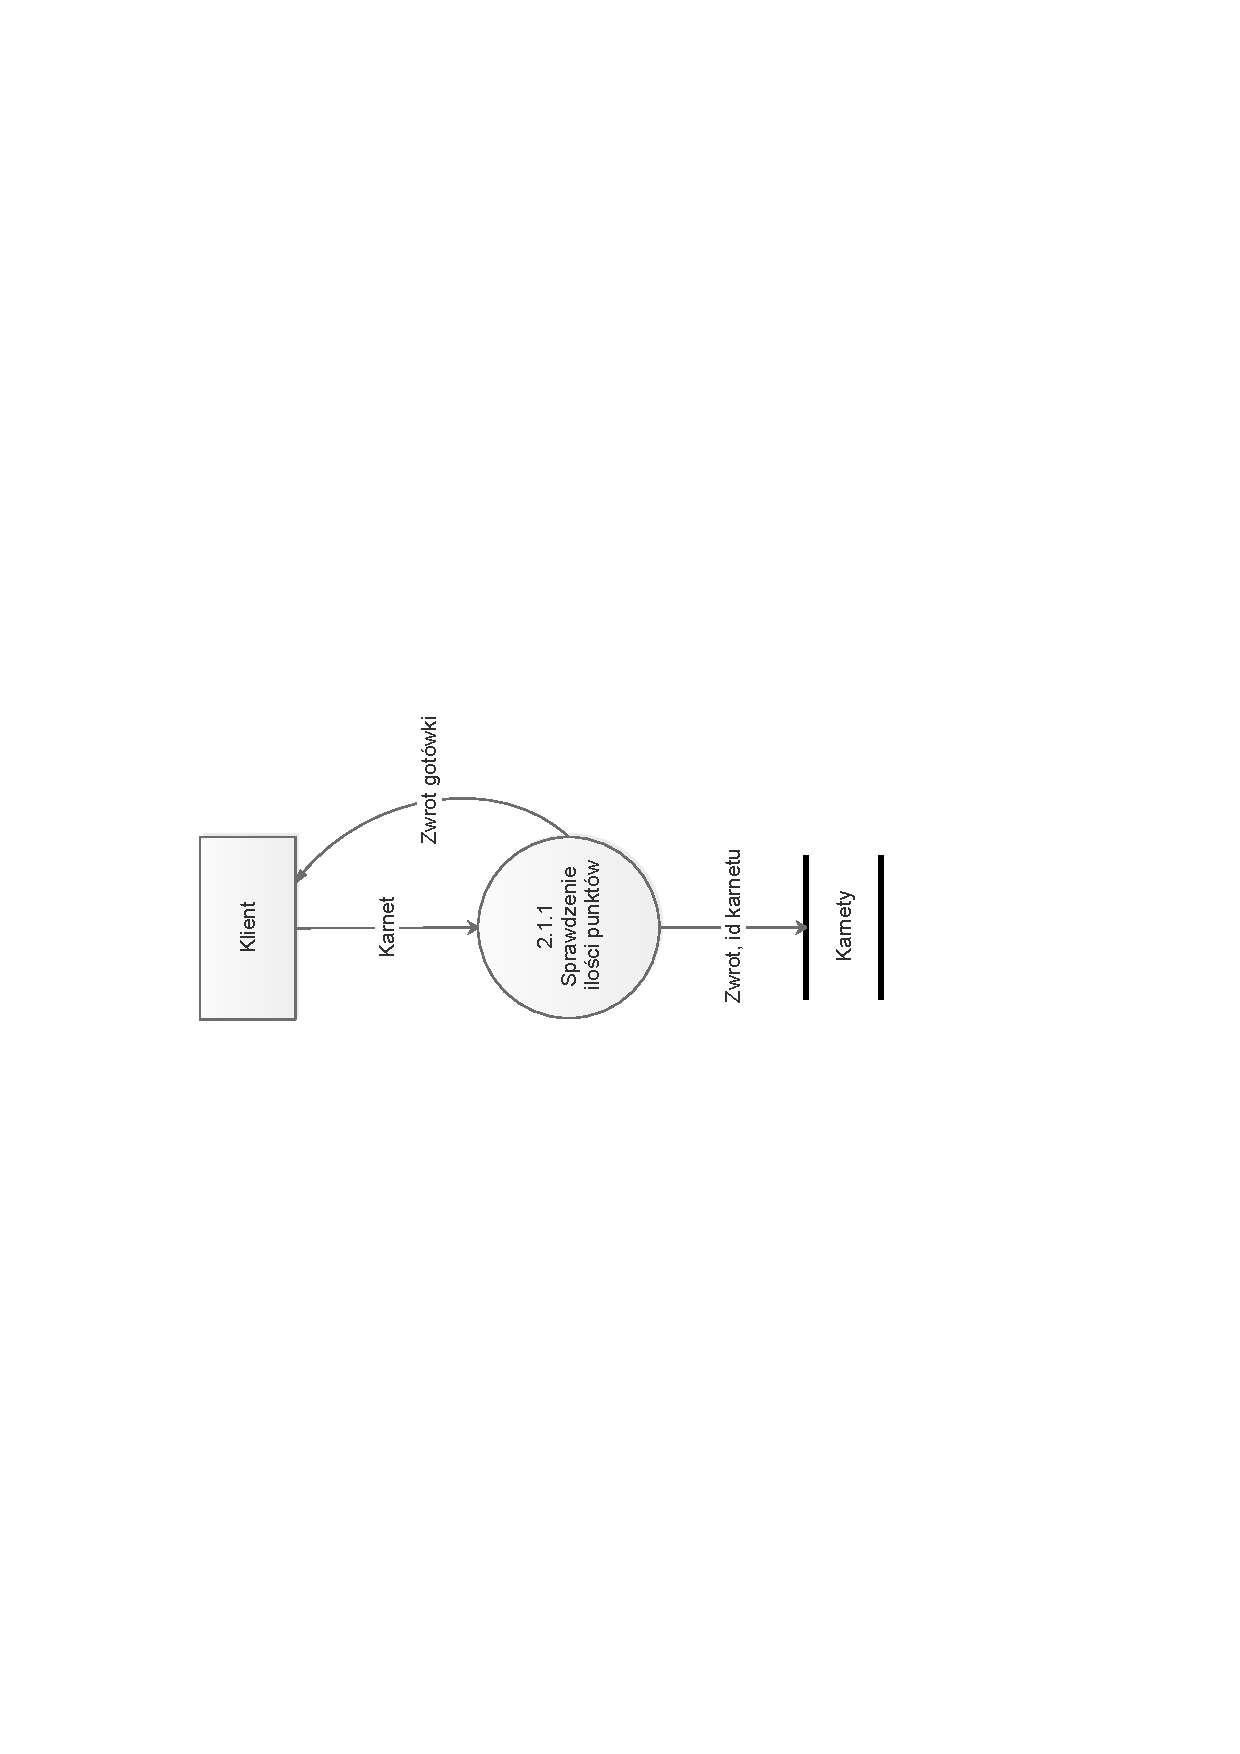
\includepdf[trim=-3cm 0 0 0]{dfd/p2/p2-zwroty-rotated}
\end{figure}

\newpage
\subsection{Wypożyczalnia sprzętu - wypożyczenie}
\begin{figure}
    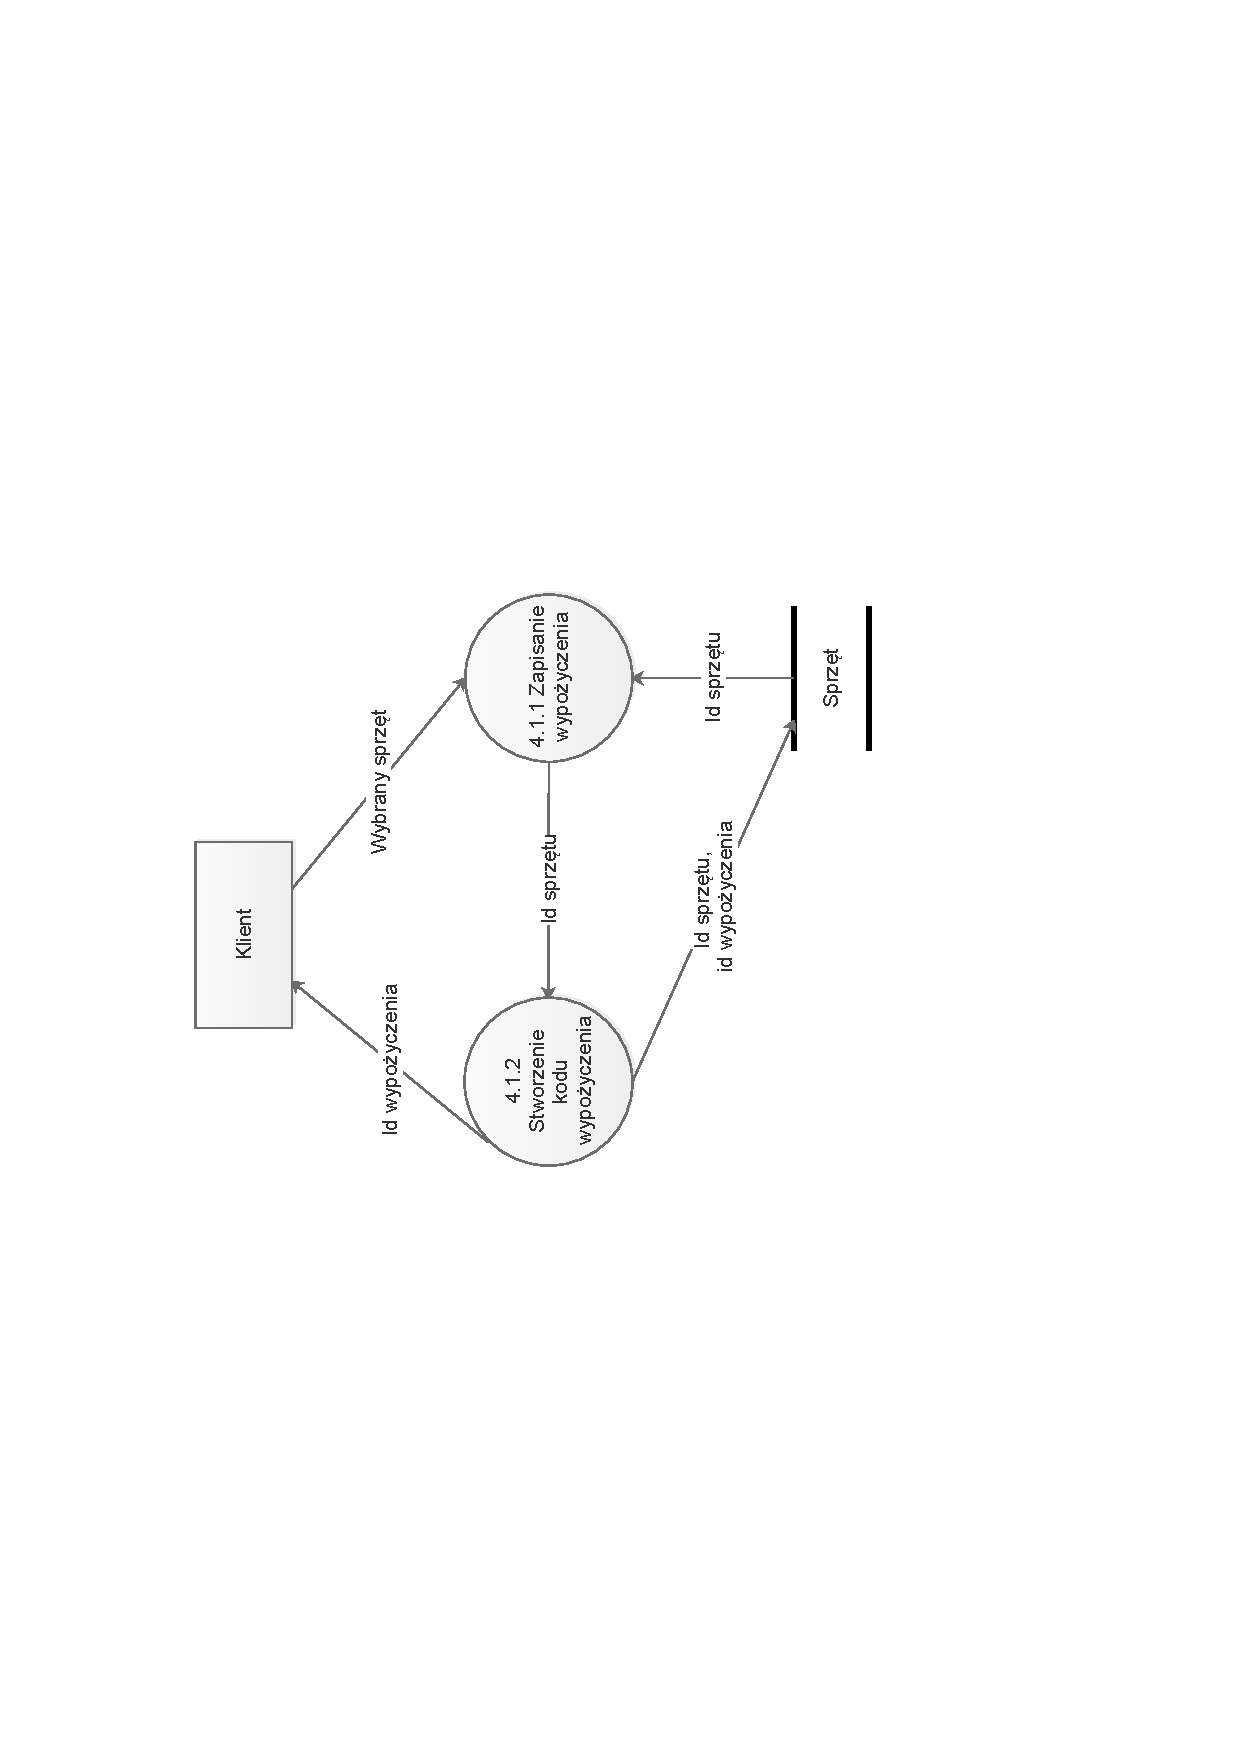
\includepdf[trim=-3cm 0 0 0]{dfd/p2/p2-wypozyczenie-rotated}
\end{figure}

\newpage
\subsection{Serwis sprzętu - serwisowanie}
\begin{figure}
    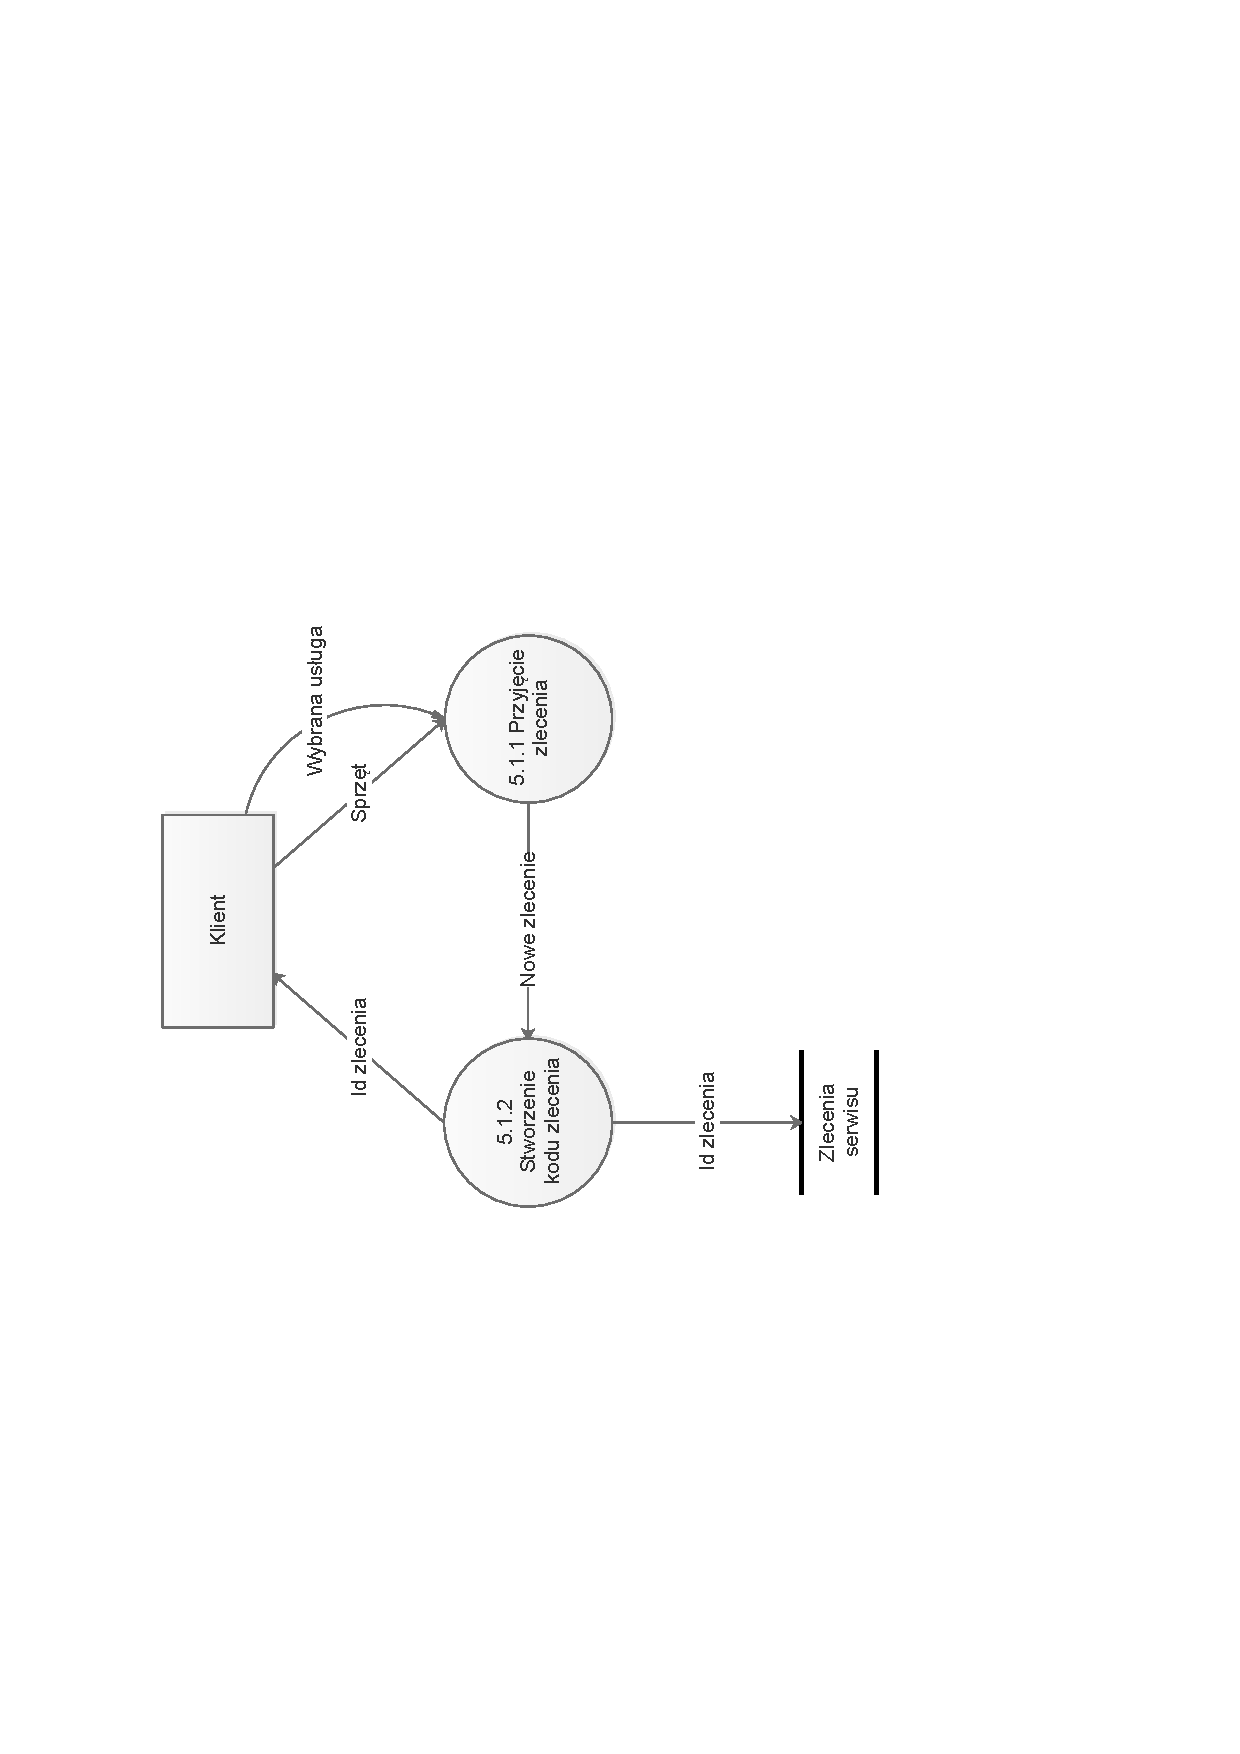
\includepdf[trim=-3cm 0 0 0]{dfd/p2/p2-serwisowanie-rotated}
\end{figure}

\newpage
\subsection{Płatność - gotówką}
\begin{figure}
    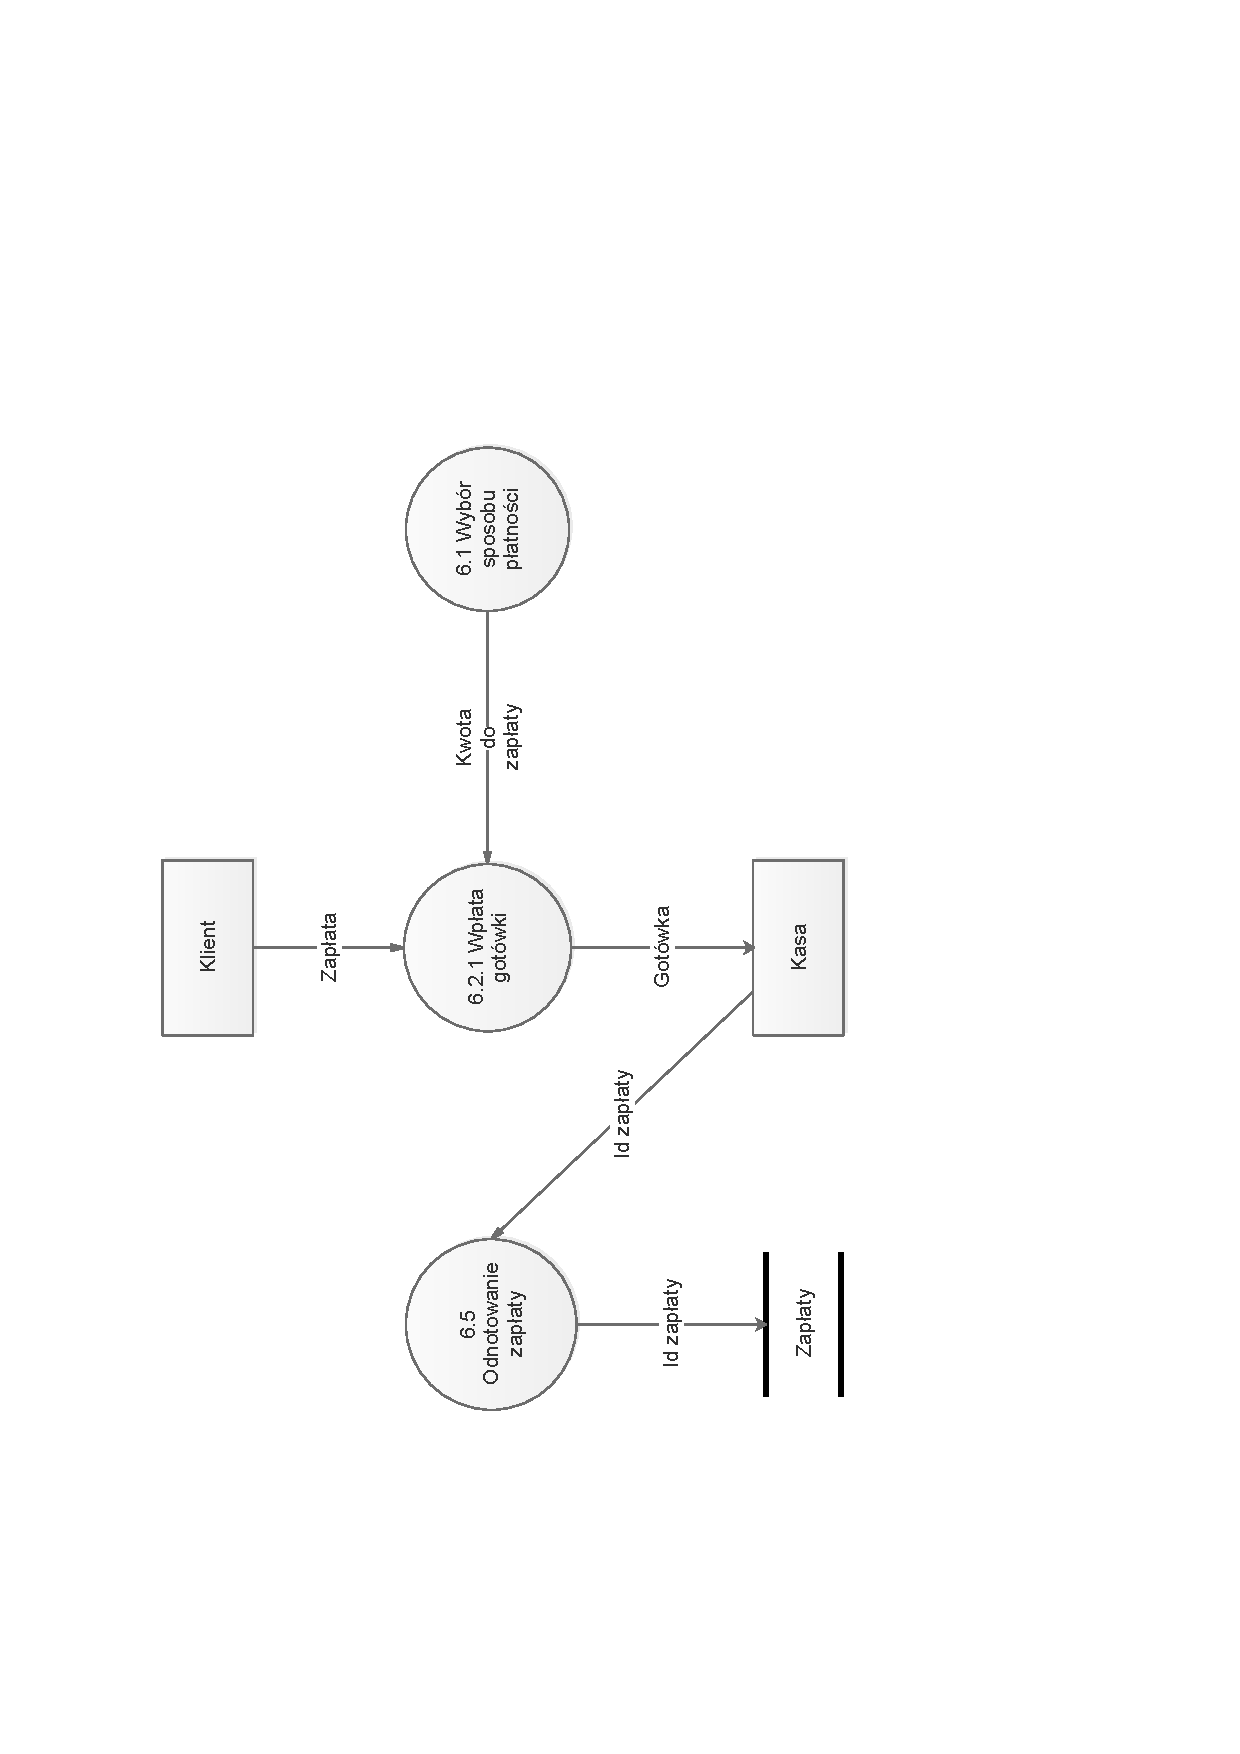
\includepdf[trim=-3cm 0 0 0]{dfd/p2/p2-cash-rotated}
\end{figure}

\newpage
\subsection{Płatność - kartą płatniczą}
\begin{figure}
    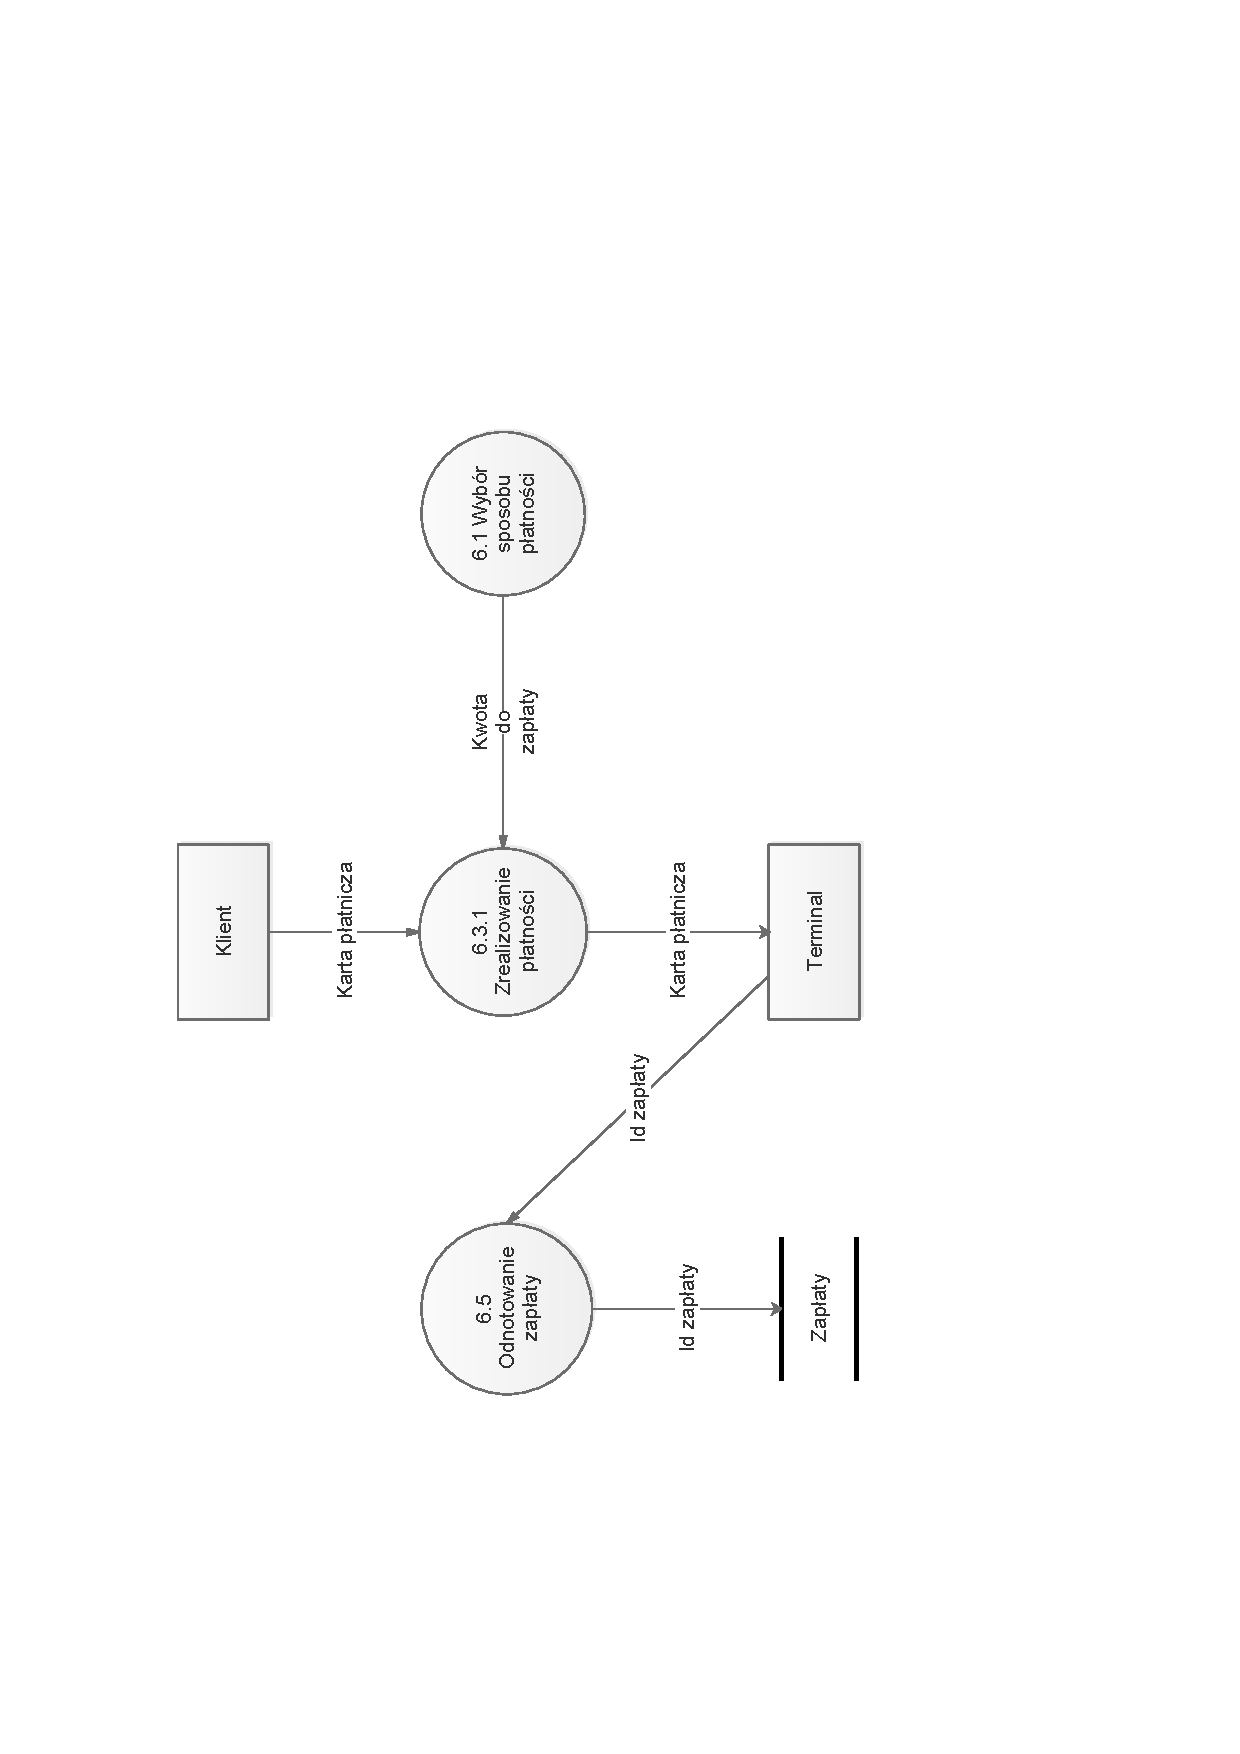
\includepdf[trim=-3cm 0 0 0]{dfd/p2/p2-debit-rotated}
\end{figure}

\newpage
\subsection{Płatność - online}
\begin{figure}
    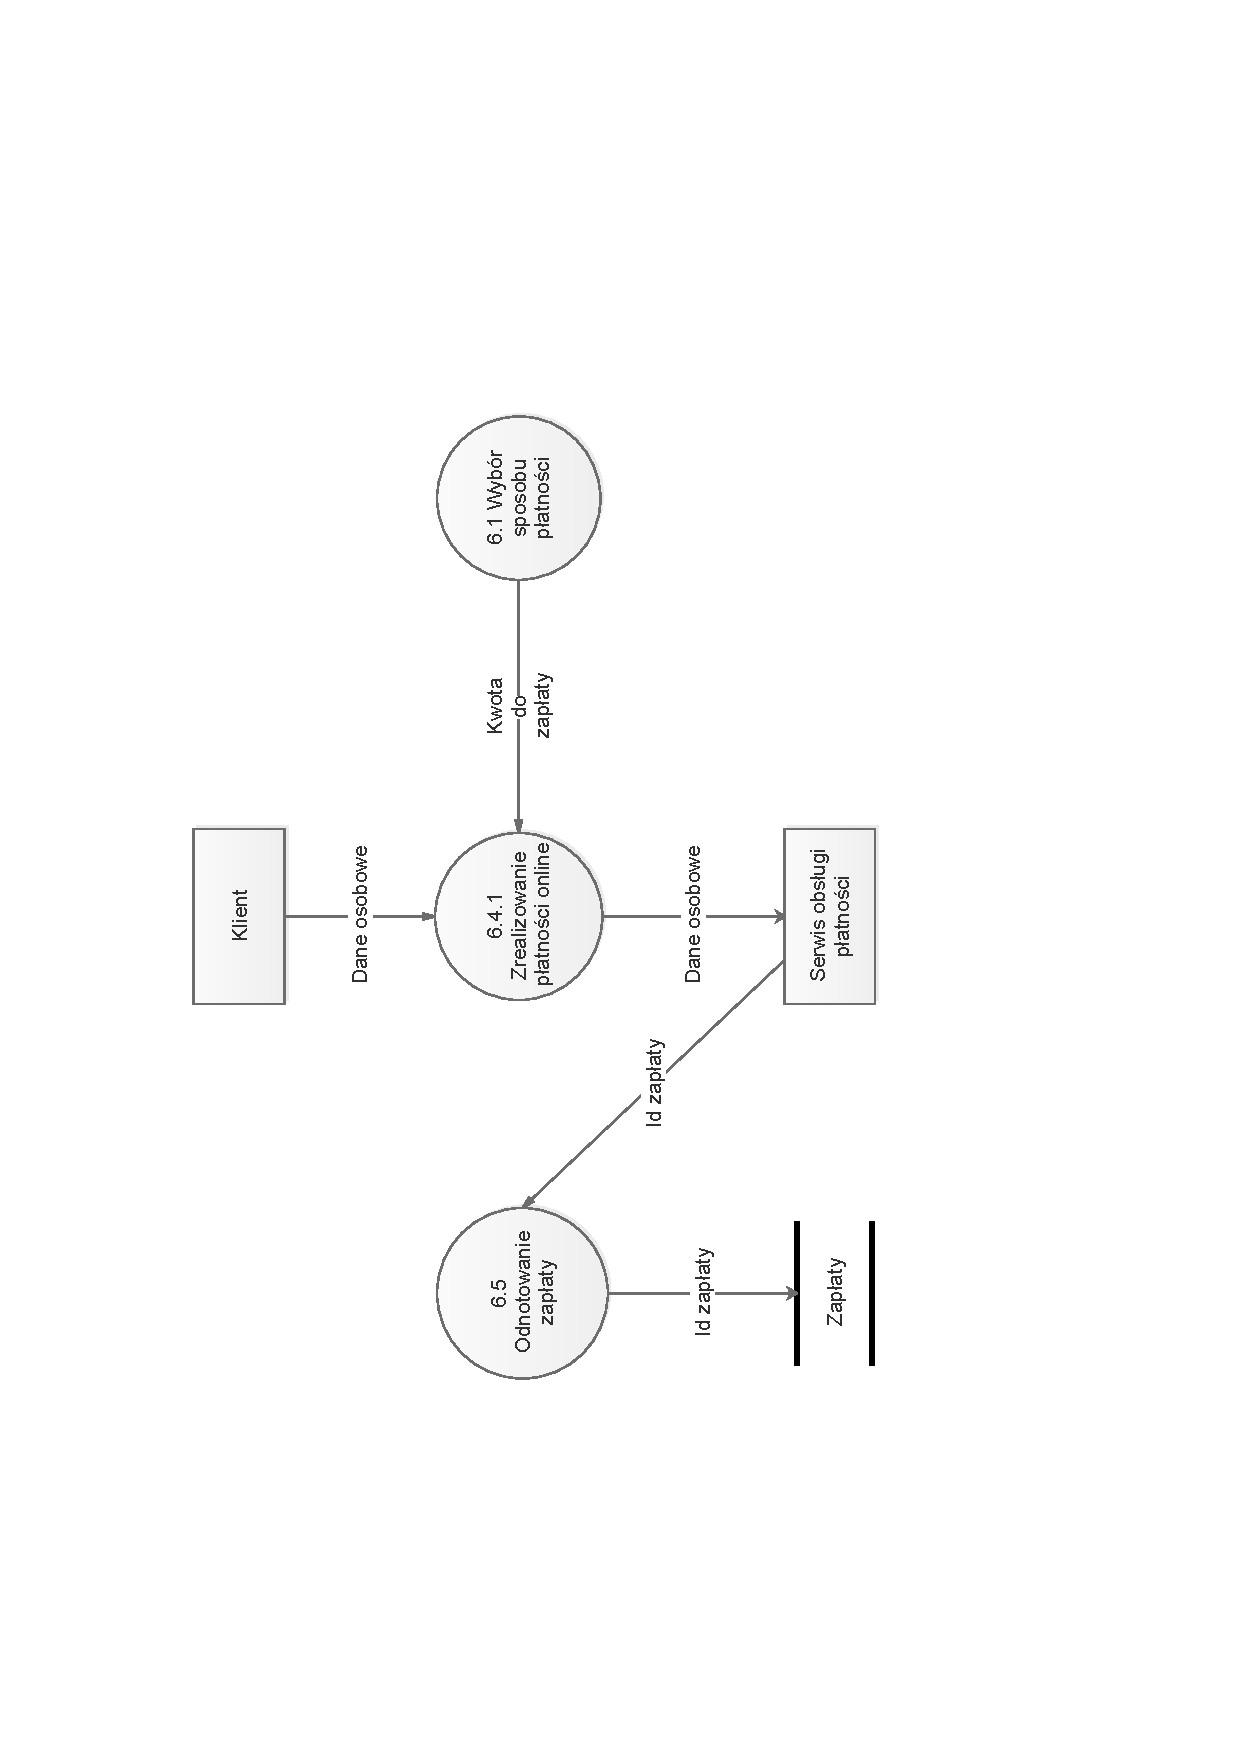
\includepdf[trim=-3cm 0 0 0]{dfd/p2/p2-online-rotated}
\end{figure}
\end{landscape}

\end{document}
